\documentclass[10pt, a4paper]{article}
\usepackage[utf8]{inputenc}
\newcommand\preamble{
    \usepackage[italian]{babel}
    \usepackage{geometry}
    \usepackage{amsmath}
    \usepackage{amssymb}
    \usepackage{graphicx}
    \usepackage{ulem}
    \geometry{margin=2cm}
    \usepackage{listings}
    \usepackage{xparse}
    \usepackage{expl3}
    \usepackage{tikz}
    \usepackage[colorlinks=true, linkcolor=blue]{hyperref}
    \usetikzlibrary{calc}
    \let\olditemize\itemize
    \renewcommand\itemize{\olditemize\setlength\itemsep{0em}}
    \geometry{a4paper, left=1.5cm, right=1.5cm, top=1cm, bottom=2cm}
}
\newcommand{\tikzmark}[1]{\tikz[baseline,remember picture] \coordinate (#1) {};}
\newcommand{\customfbox}[1]{
    \begin{center}
        \noindent\fbox{\parbox{\dimexpr\linewidth-2\fboxsep-2\fboxrule\relax}{\centering #1}}
    \end{center}
    }
\newcommand{\taylor}[3]{
    T_{#2,#3}^{#1}
}
\preamble
\begin{document}
\section{Serie Notevoli}
    \begin{center}
        \begin{tabular}{|c|p{6cm}|p{5cm}|}
            \hline
            \textbf{Tipo di Serie} & \textbf{Forma} & \textbf{Comportamento} \\
            \hline
            \textbf{Armonica Generalizzata} & $\displaystyle \sum_{n=1}^{\infty}\frac{1}{n^\alpha}$ & 
                $\begin{cases}
                    \text{Converge} & \text{se }\alpha > 1 \\
                    +\infty & \text{se }\alpha \leq 1
                \end{cases}$ \\
            \hline
            \textbf{Geometrica} & $\displaystyle \sum_{n=0}^{\infty}q^n$ (o $\sum_{n=1}^{\infty}q^n$) & 
                $\begin{cases}
                    \frac{1}{1-q} & \text{se } |q|< 1 \\
                    +\infty & \text{se } q \geq 1 \\
                    \text{Indeterminata} & \text{se } q \leq -1
                \end{cases}$ \\
            \hline
        \end{tabular}
    \end{center}
\section{Serie di Funzioni}
    Data la serie di funzioni:
    \begin{equation*}
        f(x) = \sum_{n=1}^{\infty}f_n(x)
    \end{equation*}
    \begin{enumerate}
        \item \textbf{Converge puntualmente} su $I$ se la serie converge $\forall x\in I$ e $f:I\rightarrow\mathbb{R}$
        \item \textbf{Converge assolutamente} su $I$ se la serie a termini positivi $\left(\left|f_n(x)\right|\right)$ converge $\forall x\in I$
    \end{enumerate}
    \textit{Se per qualche $x\in I$ la serie diverge o è indeterminata, bisogna restringere il dominio della funzione somma $f(x)$ all'insieme:} \begin{equation*}
        \left\{x\in I \mid \sum_{n=1}^{\infty}f_n(x) \text{ converge}\right\}
    \end{equation*}
    \subsection{Criterio di Weierstrass}
        Data una serie di funzioni, se la serie numerica a termini positivi converge:
        \begin{equation*}
            \sum_{n=1}^{\infty}\sup_{x\in I}\left|f_n(x)\right|
        \end{equation*}
        allora la serie di funzioni converge assolutamente e puntualmente (= totalmente) su $I$.
    \subsection{Strategia di Studio della Convergenza}
        \begin{enumerate}
            \item \textbf{Convergenza Puntuale:} Determinare l'insieme $I_p$ per cui $\forall x \in I_p$, la serie numerica $\sum f_n(x)$ converge. (Spesso con Criteri per serie numeriche).
            \item \textbf{Convergenza Assoluta:} Su $I_p$, studiare $\sum |f_n(x)|$.
            \item \textbf{Convergenza Uniforme/Totale:}
            \begin{itemize}
                \item Tentare il \textbf{Criterio di Weierstrass}: se $\sum \sup_{x \in I} |f_n(x)|$ converge, allora la serie converge totalmente su $I$.
                \item Se Weierstrass non funziona su $I_p$ (es. perché $\sup|f_n(x)|$ diverge, ma la serie converge comunque), cercare intervalli $J \subset I_p$ dove $\sup|f_n(x)|$ è finito e applicare Weierstrass.
                \item (Meno comune per gli esami, ma utile: altri criteri come quello di Abel-Dirichlet per convergenza uniforme.)
            \end{itemize}
        \end{enumerate}
    \customfbox{Convergenza totale $\Rightarrow$ convergenza puntuale}
    \subsection{Corollari}
        \subsubsection{Continuità della somma}
            Se:
            \begin{enumerate}
                \item Le funzioni $f_n(x)$ sono continue su $I\forall n\geq 1$
                \item La serie converge totalmente su $I$ ad $f(x)$  
            \end{enumerate}
            Allora $f(x)$ è continua su $I$.
        \subsubsection{Integrazione temine a termine}
            Data una serie di funzioni dove le funzioni $f_n(x)$ sono definite su $[a,b]$ se:
            \begin{enumerate}
                \item Le funzioni $f_n$ sono continue su $[a,b]\forall n\geq 1$
                \item La serie converge totalmente su $[a,b]$ ad $f(x)$
            \end{enumerate}
            Allora $f(x)$ è integrabile in $[a,b]$:
            \begin{equation*}
                \int_{a}^{b}f(x)dx = \sum_{n=1}^{\infty}\int_{a}^{b}f_n(x)dx
            \end{equation*}
        \subsubsection{Derivazione termine a termine}
            Data una serie di funzioni dove le funzioni $f_n(x)$ sono definite su $I$ se:
            \begin{enumerate}
                \item Le funzioni $f_n$ sono derivabili e le derivate sono funzioni continue $\forall n\geq 1$
                \item La serie $\sum_{n=1}^{\infty}f_n(x)$ converge puntualmente su $I$
                \item La serie $\sum_{n=1}^{\infty}f'_n(x)$ converge totalmente su $I$
            \end{enumerate}
            Allora $f(x)$ derivabile e:
            \begin{equation*}
                f'(x) = \sum_{n=1}^{\infty}f'_n(x) \quad \forall x\in I
            \end{equation*}
        \subsubsection{Corollario 1.34}
            Data una serie di funzioni definite su $[a,b]$ se:
            \begin{enumerate}
                \item Le funzioni $f_n(x)$ sono continue su $[a,b]\forall n\geq 1$
                \item La serie converge totalamente su $(a,b)$
            \end{enumerate}
            Allora la serie converge totalmente su $[a,b]$ e la funzione somma è continua su $[a,b]$
\section{Serie di potenze}
    La serie di funzioni
    \begin{equation*}
        \sum_{n=0}^{\infty}a_n x^n
    \end{equation*}            
    si chiama \textbf{serie di potenze di centro 0}
    \subsection{Raggio di Convergenza $R$}
        Sia $\sum_{n=0}^{\infty}a_n x^n$ una serie di potenze di centro 0. Esiste un unico $R \in [0,+\infty) \cup \{+\infty\}$, detto Raggio di Convergenza, tale che:
        \begin{itemize}
            \item Se $R=0$: la serie converge \textbf{solo in $x=0$}.
            \item Se $0<R<+\infty$:
            \begin{itemize}
                \item Converge \textbf{assolutamente} su $(-R, R)$.
                \item Converge \textbf{totalmente} su $[-K,K]$ per ogni $0 < K < R$.
                \item Non converge per $|x|>R$.
            \end{itemize}
            \item Se $R=+\infty$: la serie converge \textbf{assolutamente} su $\mathbb{R}$ e \textbf{totalmente} su $[-K,K]$ per ogni $K > 0$.
        \end{itemize}
        \textbf{Nota:} La convergenza agli estremi $x = \pm R$ deve essere studiata separatamente (convergenza puntuale).
    \subsubsection{Calcolo di $R$ (Criteri del Rapporto/Radice)}
        Sia $l = \lim_{n\to\infty} \left|\frac{a_{n+1}}{a_n}\right|$ o $l = \lim_{n\to\infty} \sqrt[n]{|a_n|}$.
        Allora il raggio di convergenza $R$ è dato da:
        \begin{equation*}
            R=\begin{cases}
                +\infty & \text{se } l = 0\\
                \frac{1}{l} & \text{se } l \in (0,+\infty)\\
                0 & \text{se } l = +\infty
            \end{cases}
        \end{equation*}
    \subsection{Insieme di Convergenza Puntuale $I_c$}
        L'insieme di convergenza puntuale si ottiene studiando la convergenza della serie negli estremi dell'intervallo $(-R, R)$.
        \begin{enumerate}
            \item Sostituire $x = R$ nella serie e studiare la convergenza della serie numerica $\sum a_n R^n$.
            \item Sostituire $x = -R$ nella serie e studiare la convergenza della serie numerica $\sum a_n (-R)^n$.
            \item L'insieme $I_c$ sarà $(-R,R)$, $[-R,R)$, $(-R,R]$ o $[-R,R]$ a seconda della convergenza agli estremi.
        \end{enumerate}
    \subsection{Proprietà della Funzione Somma $f(x) = \sum_{n=0}^{\infty}a_n x^n$}
        Sia $f(x) = \sum_{n=0}^{\infty}a_n x^n$ una serie di potenze con raggio di convergenza $R > 0$.
        \begin{itemize}
            \item \textbf{Continuità:} La funzione somma $f(x)$ è continua sull'intervallo aperto $(-R, R)$.
            \item \textbf{Derivabilità Termine a Termine:} $f(x)$ è derivabile infinite volte su $(-R, R)$, e la sua derivata $k$-esima si ottiene derivando la serie termine a termine:
            \begin{equation*}
                f^{(k)}(x) = \sum_{n=k}^{\infty}a_n \frac{n!}{(n-k)!}x^{n-k} \quad \forall x \in (-R,R)
            \end{equation*}
            Il raggio di convergenza delle serie derivate è ancora $R$.
            \item \textbf{Integrazione Termine a Termine:} $f(x)$ è integrabile su ogni intervallo compatto contenuto in $(-R, R)$, e la sua primitiva si ottiene integrando la serie termine a termine:
            \begin{equation*}
                \int f(x)dx = \sum_{n=0}^{\infty}a_n\frac{x^{n+1}}{n+1} + C
            \end{equation*}
            Il raggio di convergenza della serie integrata è ancora $R$.
            \item \textbf{Coefficienti di Maclaurin:} I coefficienti $a_n$ della serie di potenze sono legati alle derivate della funzione somma $f(x)$ nel centro ($x=0$) dalla relazione fondamentale:
            $$a_n = \frac{f^{(n)}(0)}{n!} \quad \text{o equivalentemente } f^{(n)}(0) = n!a_n$$
            Questo significa che la serie di potenze è lo sviluppo di Maclaurin della sua funzione somma.
            \item \textbf{Unicità dello Sviluppo:} Se due serie di potenze di centro 0 convergono alla stessa funzione su un intervallo $(-\delta, \delta)$ con $\delta > 0$, allora i loro coefficienti devono essere identici: $a_n = b_n$ per ogni $n$.
        \end{itemize}
\section{Convergenza e Divergenza delle Serie Numeriche}
    \subsection{Convergenza Assoluta e Semplice}
        \begin{equation*}
            \sum_{n=1}^{\infty}a_n \text{ converge assolutamente se } \sum_{n=1}^{\infty}\left|a_n\right| \text{ converge.}
        \end{equation*}
        \textbf{Teorema:} Se una serie converge assolutamente $\implies$ converge semplicemente.
    \subsection{Condizione Necessaria di Cauchy per le Serie}
        Data una serie qualsiasi $\sum_{n=1}^{\infty}a_n$:
        \begin{equation*}
            \lim_{n\rightarrow+\infty}a_n = \begin{cases}
                0 & \Rightarrow \text{la serie \textbf{può} convergere o divergere (caso dubbio)} \\
                \neq 0 \text{ o non esiste} & \Rightarrow \text{la serie \textbf{diverge} sicuramente}
            \end{cases}
        \end{equation*}
        \textbf{Nota:} Questa condizione è \textbf{necessaria ma non sufficiente} alla convergenza della serie.
    
    \newpage
    \subsection{Criteri di Convergenza/Divergenza per Serie a Termini Definitivamente Positivi}
        (\textit{Ovvero $\exists n_0$ tale che $a_n \geq 0$ per ogni $n \geq n_0$})
        \begin{itemize}
            \item \textbf{Criterio del Rapporto} (Utile con fattoriali $n!$ o potenze con $n$ all'esponente):
            Sia $l = \lim_{n\rightarrow +\infty}\frac{a_{n+1}}{a_n}$.
            \begin{enumerate}
                \item Se $l<1 \Rightarrow$ la serie converge.
                \item Se $l>1 \Rightarrow$ la serie diverge.
                \item Se $l=1 \Rightarrow$ il criterio non fornisce informazioni (la serie può convergere o divergere).
            \end{enumerate}

            \item \textbf{Criterio della Radice} (Utile con potenze $n$-esime come $(f(n))^n$):
            Sia $l = \lim_{n\rightarrow+\infty}\sqrt[n]{a_n}$.
            \begin{enumerate}
                \item Se $l<1 \Rightarrow$ la serie converge.
                \item Se $l>1 \Rightarrow$ la serie diverge.
                \item Se $l=1 \Rightarrow$ il criterio non fornisce informazioni.
            \end{enumerate}

            \item \textbf{Criterio del Confronto}: Supponiamo che $0 \leq a_n \leq b_n$ definitivamente.
            \begin{itemize}
                \item Se $\sum b_n$ converge $\Rightarrow$ $\sum a_n$ converge.
                \item Se $\sum a_n$ diverge $\Rightarrow$ $\sum b_n$ diverge.
            \end{itemize}

            \item \textbf{Criterio del Confronto Asintotico}:
            Siano $a_n, b_n > 0$ definitivamente. Sia $L = \lim_{n\rightarrow +\infty}\frac{a_n}{b_n}$.
            \begin{equation*}
                \begin{cases}
                    L \in (0,+\infty) & \Rightarrow \sum a_n \text{ e } \sum b_n \text{ hanno lo stesso comportamento (convergenza/divergenza)} \\
                    L = 0 & \Rightarrow \text{Se } \sum b_n \text{ converge} \Rightarrow \sum a_n \text{ converge (se } \sum b_n \text{ diverge, nulla si può dire)} \\
                    L = +\infty & \Rightarrow \text{Se } \sum b_n \text{ diverge} \Rightarrow \sum a_n \text{ diverge (se } \sum b_n \text{ converge, nulla si può dire)}
                \end{cases}
            \end{equation*}
            \textit{Suggerimento per scegliere $b_n$}: Prendi i termini di grado maggiore in numeratore e denominatore di $a_n$. (Es. $a_n=\frac{n+1}{n^2+3} \Rightarrow b_n=\frac{n}{n^2}=\frac{1}{n}$)

            \item \textbf{Test dell'Integrale}:
            Sia $f: [1, +\infty) \to \mathbb{R}$ una funzione positiva e decrescente.
            Posto $a_n = f(n)$ per ogni $n \geq 1$, allora:
            \begin{equation*}
                \sum_{n=1}^{\infty} a_n \text{ converge } \iff \int_{1}^{+\infty} f(x)dx \text{ converge}
            \end{equation*}
            Inoltre, valgono le disuguaglianze per la somma $S$ della serie e l'integrale improprio $I$:
            \begin{equation*}
                \int_{1}^{+\infty} f(x)dx \leq S \leq a_1 + \int_{1}^{+\infty} f(x)dx
            \end{equation*}
        \end{itemize}

    \subsection{Criteri di Convergenza per Serie a Termini di Segno Alterno}
        \begin{itemize}
            \item \textbf{Criterio di Leibniz} (per serie del tipo $\sum_{n=1}^{\infty}(-1)^n a_n$ o $\sum_{n=1}^{\infty}(-1)^{n+1} a_n$):
            Se la successione $a_n$ soddisfa le seguenti condizioni:
            \begin{enumerate}
                \item $\lim_{n\rightarrow+\infty}a_n=0$
                \item $a_n$ è decrescente definitivamente ($a_{n+1} \leq a_n$ per $n \geq n_0$)
            \end{enumerate}
            allora la serie converge \textbf{semplicemente}.

            \item \textbf{Stima dell'Errore per Serie di Leibniz}:
            Se una serie converge per il criterio di Leibniz a una somma $S$, e $S_N$ è la somma parziale fino all'N-esimo termine, allora l'errore commesso è limitato dal primo termine tralasciato:
            $\left|S - S_N\right| \leq a_{N+1}$.

            \item \textbf{Criterio di Dirichlet (per serie numeriche)}:
            Consideriamo una serie $\sum_{n=1}^{\infty}a_nb_n$. Se valgono le seguenti condizioni:
            \begin{enumerate}
                \item Le somme parziali di $\sum a_n$ sono limitate: $\exists M>0 \mid \left|\sum_{k=1}^{N}a_k\right|\leq M \quad \forall N\geq 1$.
                \item La successione $b_n$ è monotona (crescente o decrescente) definitivamente.
                \item $\lim_{n\rightarrow+\infty}b_n=0$.
            \end{enumerate}
            Allora la serie $\sum_{n=1}^{\infty}a_nb_n$ converge.
            \textit{(Questo criterio è più generale di Leibniz, che è un caso particolare di Dirichlet con $a_n = (-1)^n$ o $(-1)^{n+1}$)}.
        \end{itemize}

    \begin{center}
        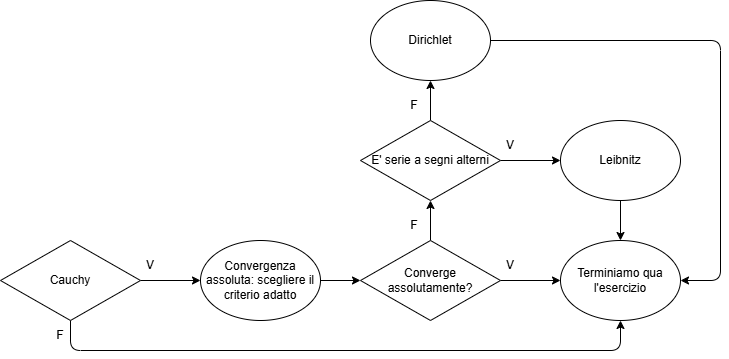
\includegraphics[width=.8\textwidth]{Images/convergenzaflowchart.png}
    \end{center}

    \newpage
    \subsection{Esercizio d'esame}
        \textit{Stabilire se le seguenti serie sono a termini positivi e convergono semplicemente e/o assolutamente.}
        \begin{enumerate}
            \item $\sum_{n=1}^{+\infty}(-1)^{n+1}\sin\left(\frac{1001}{\sqrt{n}}\right)$ 
            \begin{enumerate}
                \item \textbf{Cauchy}: $\lim_{n\rightarrow+\infty}\sin\left(\frac{1001}{\sqrt{n}}\right)=\sin\left(\frac{1001}{\infty}\right)=\sin(0)=0$
                \item \textbf{Convergenza assoluta}: $\sum_{n=1}^{+\infty}\left|(-1)^{n+1}\sin\left(\frac{1001}{\sqrt{n}}\right)\right|=\sum_{n=1}^{+\infty}\sin\left(\frac{1001}{\sqrt{n}}\right)$ 
                    \begin{enumerate}
                        \item \textbf{Criterio di confronto asintotico}: \scriptsize$a_n = \sin\left(\frac{1001}{\sqrt{n}}\right), b_n = \frac{1001}{\sqrt{n}} \rightarrow \lim_{n\rightarrow+\infty}\frac{a_n}{b_n}=\lim_{n\rightarrow+\infty}\frac{\sin\left(\frac{1001}{\sqrt{n}}\right)}{\frac{1001}{\sqrt{n}}}=1$\normalsize \\ $\rightarrow$ $a_n$ e $b_n$ hanno lo stesso comportamento.
                        \item \textbf{Serie armonica generalizzata}: $\frac{1001}{\sqrt{n}}\rightarrow\alpha=\frac{1}{2}\Rightarrow$ diverge
                        \item Grazie al punto precedente possiamo dire che la serie originale non converge assolutamente (perchè è una serie a segno alternato), ora procederemo con Leibnitz
                    \end{enumerate}
                \item \textbf{Criterio di Leibnitz}: 
                    \begin{enumerate}
                        \item $\lim_{n\rightarrow+\infty}\sin\left(\frac{1001}{\sqrt{n}}\right)=0?$ L'abbiamo già fatto nel punto (a)
                        \item Decrescente? \begin{enumerate}
                        \item $a_n'=\cos\left(\frac{1001}{\sqrt{n}}\right)\cdot\left(-\frac{1001}{2\sqrt{n}}\cdot\frac{1}{n}\right)=\cos\left(\frac{1001}{\sqrt{n}}\right)\cdot\left(-\frac{1001}{2n^{\frac{1}{2}}n}\right)=\cos\left(\frac{1001}{\sqrt{n}}\right)\cdot\left(-\frac{1001}{2n^{\frac{3}{2}}}\right)$
                        \item $a'_n>0\begin{cases}
                                \cos\left(\frac{1001}{\sqrt{n}}\right)>0\rightarrow -\frac{\pi}{2}\leq\frac{1001}{\sqrt{n}}\leq\frac{\pi}{2}\rightarrow n \geq 406269\\
                                \left(-\frac{1001}{2n^{\frac{3}{2}}}\right)>0\rightarrow \text{Impossibile sarà sempre negativo perchè } n\geq 1
                            \end{cases}$
                        \item Quindi sapendo che la serie è decrescente con $n\geq 406269$, possiamo dire che anche questo requisito è soddisfatto
                    \end{enumerate}
                \end{enumerate}
                \item \textbf{Conclusione}: visto che la serie soddisfa tutti i requisiti del criterio di Leibnitz allora converge semplicemente.
            \end{enumerate}
            \item $\sum_{n=1}^{+\infty}\frac{n(3-(\cos n)^2)}{n^3+2n+1}$ \begin{enumerate}
                \item \textbf{Cauchy}: $\lim_{n\rightarrow+\infty}\frac{n(3-(\cos n)^2)}{n^3+2n+1}=0$
                \item \textbf{Convergenza assoluta}: $\sum_{n=1}^{+\infty}\left|\frac{n(3-(\cos n)^2)}{n^3+2n+1}\right|$ \begin{enumerate}
                    \item \textbf{Criterio di confronto asintotico:} $a_n=\frac{n(3-(\cos n)^2)}{n^3+2n+1}, b_n=\frac{1}{n^2}$
                    \begin{equation*}
                            \lim_{n\rightarrow+\infty}\frac{a_n}{b_n}=\lim_{n\rightarrow+\infty}\frac{\frac{n(3-(\cos n)^2)}{n^3+2n+1}}{\frac{1}{n^2}}=\lim_{n\rightarrow+\infty}\frac{n^3\left(3-(\cos n)^2\right)}{n^3+2n+1} = \lim_{n\rightarrow+\infty}\frac{\left(3-(\cos n)^2\right)}{1+\frac{2}{n^2}+\frac{1}{n^3}}=3
                    \end{equation*}
                    \item \textbf{Serie armonica generalizzata}: $\frac{1}{n^2}\rightarrow  \alpha=2\Rightarrow b_n$ converge
                \end{enumerate}
                \item \textbf{Conclusione:} Grazie al punto precedente e al teorema del confronto possiamo affermare che la serie converge assolutamente e, di conseguenza, semplicemente.
            \end{enumerate}
            \item \textit{Data la serie di potenze} $\sum_{n=1}^{+\infty}\frac{2^n+3^{-n}}{n^2}x^n$ \textit{determinare il raggio di convergenza $\rho$ e l'insieme di convergenza puntuale I}. \begin{enumerate}
                \item \textbf{Cauchy}: $\lim_{n\rightarrow+\infty}\frac{2^n+3^{-n}}{n^2}=0$
                \item \textbf{Convergenza assoluta}: $\sum_{n=1}^{+\infty}\left|\frac{2^n+3^{-n}}{n^2}\right|$
                \customfbox{Le forme indeterminate del tipo $f(n)^{g(n)}=\{0^0, \infty^0, 1^\infty\}$ si risolvono $f(n)^{g(n)}=e^{g(n)\ln\left(f(n)\right)}$}
                \begin{enumerate}
                    \item \textbf{Criterio della radice}: \begin{equation*}
                        \begin{split}
                            \lim_{n\rightarrow+\infty}\sqrt[n]{\left|\frac{2^n+3^{-n}}{n^2}\right|}&=\lim_{n\rightarrow+\infty}\left(\left|\frac{2^n}{n^2}\right|\right)^{\frac{1}{n}}=\lim_{n\rightarrow+\infty}e^{\frac{1}{n}\ln\left(\frac{2^n}{n^2}\right)}\\
                            &=\lim_{n\rightarrow+\infty}e^{\frac{1}{n}\left(\ln\left({2^n}\right)-\ln\left({n^2}\right)\right)}=\lim_{n\rightarrow+\infty}e^{\frac{1}{n}\left(n\ln\left({2}\right)-2\ln\left({n}\right)\right)}\\
                            &=\lim_{n\rightarrow+\infty}e^{\ln\left({2}\right)-\frac{2\ln\left({n}\right)}{n}}=e^{\ln(2)}=2
                        \end{split}
                    \end{equation*}
                    \item \textbf{Determiniamo $\rho$}: $\rho=\frac{1}{2}$ per definizione\\
                    \item \textbf{Determinare $I_c$}: \begin{enumerate}
                        \item si "creano" due serie diverse usando l'intervallo $\left[x_0-p,x_0+p\right]$ e sostituendo $x$ con entrambi gli estremi: \begin{equation*}
                            \begin{split}
                                &\sum_{n=1}^{+\infty}\frac{2^n+3^{-n}}{n^2}\left(x_0-p\right)^n\\
                                &\sum_{n=1}^{+\infty}\frac{2^n+3^{-n}}{n^2}\left(x_0+p\right)^n
                            \end{split}
                        \end{equation*}
                        \item \textbf{Studiamo la convergenza di entrambe}: \begin{equation*}
                            \begin{split}
                                &\frac{2^n+3^{-n}}{n^2}\left(0-\frac{1}{2}\right)^n=\frac{\left(2^n+3^{-n}\right)\left(-\frac{1}{2}\right)^n}{n^2}=\frac{(-1)^n+\left(-\frac{1}{6}\right)^n}{n^2}\\
                                &\rightarrow\left|\frac{(-1)^n+\left(-\frac{1}{6}\right)^n}{n^2}\right|=\frac{1+\left(\frac{1}{6}\right)^n}{n^2}\\
                                &=\frac{1}{n^2}+\frac{\left(\frac{1}{6}\right)^n}{n^2}=\begin{cases}
                                    \frac{1}{n^2} & \text{serie armonica, converge}\\
                                    \frac{\left(\frac{1}{6}\right)^n}{n^2}\rightarrow \frac{\frac{\left(\frac{1}{6}\right)^n}{n^2}}{\left(\frac{1}{6}\right)^n} & \scriptsize\text{per confronto asintoto } b_n \text{ converge perchè serie geometrica}\normalsize
                                \end{cases}\\
                                &\frac{2^n+3^{-n}}{n^2}\left(0+\frac{1}{2}\right)^n \rightarrow \text{analogamente a quella di sopra converge}
                            \end{split}                            
                        \end{equation*}
                        \item Quindi, visto che converge per entrambi gli estremi $I_c=\left[-\frac{1}{2},\frac{1}{2}\right]$
                    \end{enumerate}
                \end{enumerate}
            \end{enumerate}
        \end{enumerate}
\section{Polinomio di McLaurin}
    Consideriamo:
    \begin{equation*}
        c_k = \frac{f^{(k)}(0)}{k!}
    \end{equation*}
    \begin{equation*}
        f^{(k)}(0) = c_k\cdot k!
    \end{equation*}
    \begin{equation*}
        P_k(x)=f(0)+\sum_{n=1}^{k}c_k x^k
    \end{equation*}
    \begin{center}
        \begin{tabular}{|p{4cm}|p{10.5cm}|}
            \hline
            \textbf{Funzione $f(x)$} & \textbf{Serie di Maclaurin} \\
            \hline
            $e^x$ & $\displaystyle \sum_{n=0}^{\infty} \frac{x^n}{n!} = 1 + x + \frac{x^2}{2!} + \frac{x^3}{3!} + \dots$ \\
            \hline
            $\sin(x)$ & $\displaystyle \sum_{n=0}^{\infty} \frac{(-1)^n}{(2n+1)!}x^{2n+1} = x - \frac{x^3}{3!} + \frac{x^5}{5!} - \frac{x^7}{7!} + \dots$ \\
            \hline
            $\cos(x)$ & $\displaystyle \sum_{n=0}^{\infty} \frac{(-1)^n}{(2n)!}x^{2n} = 1 - \frac{x^2}{2!} + \frac{x^4}{4!} - \frac{x^6}{6!} + \dots$ \\
            \hline
            $\frac{1}{1-x}$ (Serie Geometrica) & $\displaystyle \sum_{n=0}^{\infty} x^n = 1 + x + x^2 + x^3 + \dots$ \\
            \hline
            $\ln(1+x)$ & $\displaystyle \sum_{n=1}^{\infty} \frac{(-1)^{n+1}}{n}x^n = x - \frac{x^2}{2} + \frac{x^3}{3} - \frac{x^4}{4} + \dots$ \\
            \hline
            $\arctan(x)$ & $\displaystyle \sum_{n=0}^{\infty} \frac{(-1)^n}{2n+1}x^{2n+1} = x - \frac{x^3}{3} + \frac{x^5}{5} - \frac{x^7}{7} + \dots$ \\
            \hline
            $(1+x)^\alpha$ (Serie Binomiale) & $\displaystyle \sum_{n=0}^{\infty} \binom{\alpha}{n}x^n = 1 + \alpha x + \frac{\alpha(\alpha-1)}{2!}x^2 + \dots$ \\
            & \quad dove $\binom{\alpha}{n} = \frac{\alpha(\alpha-1)\dots(\alpha-n+1)}{n!}$ \\
            \hline
            $(1-x)^{-k}$ & $\displaystyle \sum_{n=0}^{\infty} \binom{n+k-1}{n}x^n = 1 + kx + \frac{k(k+1)}{2!}x^2 + \dots$ \\
            & (Questo è un caso speciale della serie binomiale con $\alpha = -k$) \\
            \hline
        \end{tabular}
    \end{center}
    \newpage
    \subsection{Esercizio da esame}
        \begin{itemize}
            \item \textit{Data la funzione $f(x)=x(e^x-1)+\ln(1+x^2)+\sin(2x)$, calcolarne il polinomio di McLaurin di ordine 4} \begin{enumerate}
                \item Dividiamo $f(x)$ in polinomi che contengono le funzioni elementari quindi avremo: \begin{itemize}
                    \item $x(e^x-1)=x\left(1+x+\frac{1}{2}x^2+\frac{1}{3!}x^3-1\right)=x^2+\frac{x^3}{2}+\frac{x^4}{3!}$
                    \item $\ln(1+x^2)=\left(x^2-\frac{(x^2)^2}{2}\right)=x^2-\frac{x^4}{2}$
                    \item $\sin(2x)=2\left(x-\frac{x^3}{3!}\right)=2x-\frac{(2x)^3}{3!}$
                \end{itemize}
                \item Costruiamo una tabella di questo tipo: 
                \begin{center}
                    \begin{tabular}{| c | c | c | c | c |}
                        \hline
                        \textbf{Ordine} & $x(e^x-1)$ & $\ln(1+x^2)$ & $\sin(2x)$ & \textbf{Somma}\\
                        \hline
                        1 & / & / & $2x$ & $2x$ \\
                        \hline
                        2 & $x^2$ & $x^2$ & / & $2x^2$\\
                        \hline
                        3 & $\frac{x^3}{2}$ & / & $-\frac{(2x)^3}{3!}$ & $-\frac{5x^3}{6}$\\
                        \hline
                        4 & $\frac{x^4}{3!}$ & $-\frac{x^4}{2}$ & / & $-\frac{x^4}{3}$\\
                        \hline
                    \end{tabular}
                \end{center}
                Dove andiamo a prendere gli elementi di ciascun polinomio dell'ordine indicato nella prima colonna ed eseguiamo la somma della riga nell'ultima colonna.
                \item Poi costruiamo il polinomio $P_4(x)$ sommando l'ultima colonna: $P_4(x)=2x+2x^2-\frac{5x^3}{6}-\frac{x^4}{3}$
            \end{enumerate}
            \item \textit{Scrivere il resto di Lagrange $R_1(x)$ di ordine 1 (con centro in 0) della funzione $g(x)=\cos(x^2)+\sin(3x)$ e determinarne una stima per $x\in(0,\frac{1}{4}]$} \begin{enumerate}
                \item %FAI QUESTO
            \end{enumerate}
        \end{itemize}
\section{Formula di Taylor}
    \customfbox{$f^{(n)}$ indica l'ordine di derivazione $n$-esimo}
    Data una funzione $f:I\rightarrow\mathbb{R}$ definita su un intervallo $I$ e derivabile infinite volte ($C^{\infty}$)
    \subsection{Polinomio di Taylor di $f$ centrato in $x_0$ di ordine $n$}
        \begin{equation*}
            \taylor{f}{x_0}{n}(x) = f(x_0)+f'(x_0)(x-x_0)+f''(x_0)\frac{(x-x_0)^2}{2!}+\ldots+f^{(n)}(x_0)\frac{(x-x_0)^n}{n!}
        \end{equation*}
    \subsection{Formula di Taylor con resto di Lagrange}
        \begin{equation*}
            \begin{split}
                &f(x) = \taylor{f}{x_0}{n}(x) + R_nf(x)\\
                &R_nf(x) = \frac{f^{(n+1)}(c_n)(x-x_0)^{n+1}}{(n+1)!} \text{ con } c_n\in\{x_0,x\}
            \end{split}
        \end{equation*}
        Se $x=b$ e $x_0$ è vicino a $b$, $\taylor{f}{x_0}{n}(b)$ approssima $f(b)$ e $\left|f(b)-\taylor{f}{x_0}{n}(b)\right| = \left|R_nf(b)\right|$
    \subsection{Formula di Taylor con resti di Peano}
        \begin{equation*}
                f(x)= \taylor{f}{x_0}{n}(x) + (x-x_0)^n + \varepsilon(x-x_0) \text{ con } \lim_{x\rightarrow x_0} \varepsilon(x-x_0) = 0
        \end{equation*}
    \subsection{Unicità del Polinomio di Taylor}
    \begin{equation*}
        f(x)=(a_0+a_1(x-x_0)+\ldots+a_n(x-x_0)^n)+\varepsilon(x-x_0)(x-x_0)^n
    \end{equation*}
    Dove $a_0,a_1,\ldots,a_n\in\mathbb{R}$ e $\lim_{x\rightarrow x_0}\varepsilon(x-x_0)=0$ allora:
    \begin{equation*}
        a_k = \frac{f^{(k)}(x_0)}{k!}
    \end{equation*}
    \begin{center}
        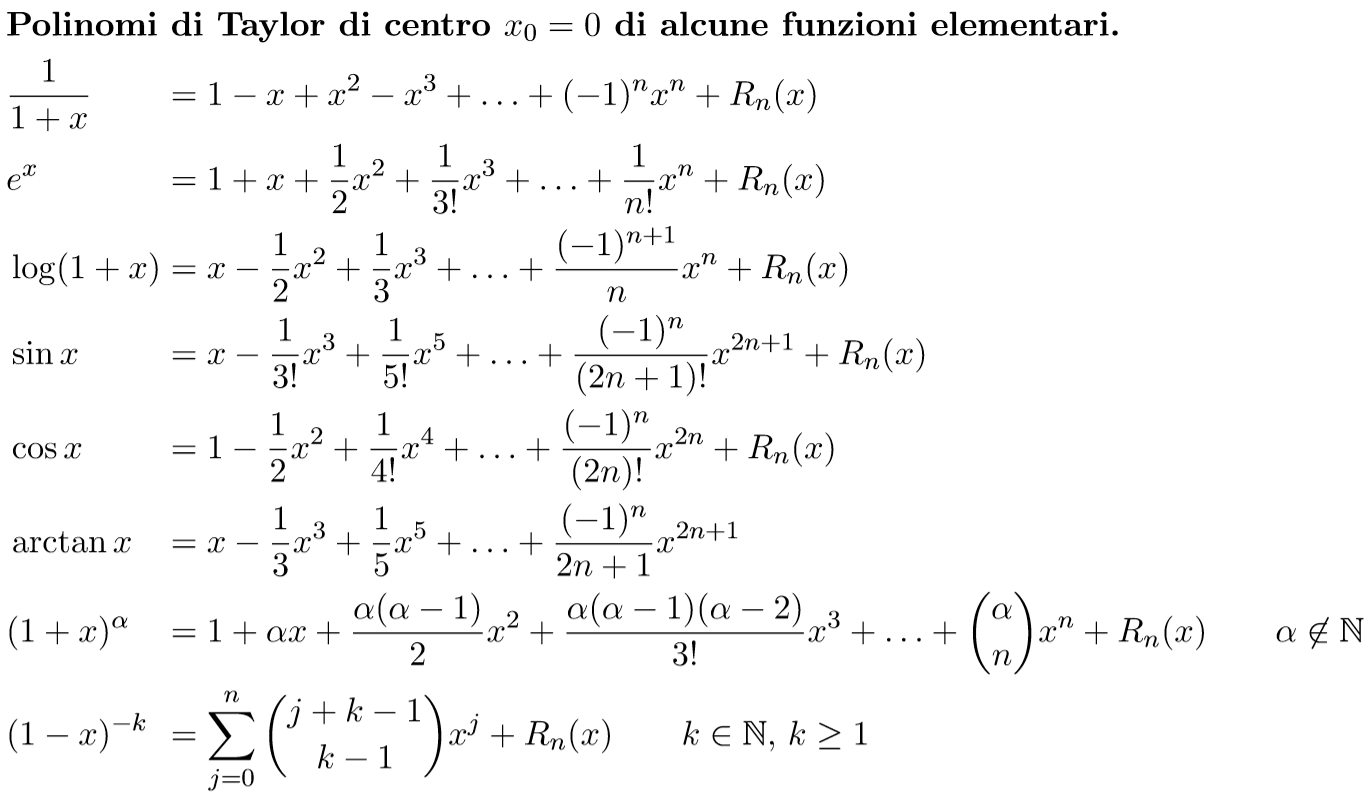
\includegraphics[width=0.8\textwidth]{Images/serieditaylor.png}
    \end{center}
\newpage
\section{Fourier}
    \subsection{Coefficienti}
        Data una funzione $f$ periodica di periodo $T$, i coefficienti di Fourier sono dati da:
        \begin{equation*}
            \hat{f_k}=\frac{1}{T}\int_{-\frac{T}{2}}^{\frac{T}{2}}f(x)e^{-i\frac{2\pi}{T}kx} \qquad k\in\mathbb{Z}
        \end{equation*}
        E usando l'identità di Eulero:
        \begin{equation*}
            \hat{f_k}=\left(\frac{1}{T}\int_{-\frac{T}{2}}^{\frac{T}{2}}f(x)\cos\left(\frac{2\pi}{T}kx\right)dx\right)-i\left(\frac{1}{T}\int_{-\frac{T}{2}}^{\frac{T}{2}}f(x)\sin\left(\frac{2\pi}{T}kx\right)dx\right)
        \end{equation*}
        \subsubsection{Coefficienti reali}
        \begin{itemize}
            \item $a_k=\hat{f_k}+\hat{f}_{-k}=\frac{2}{T}\int_{-\frac{T}{2}}^{\frac{T}{2}}f(x)\cos\left(\frac{2\pi}{T}kx\right)dx$
            \item $b_k=i(\hat{f_k}+\hat{f}_{-k})=\frac{2}{T}\int_{-\frac{T}{2}}^{\frac{T}{2}}f(x)\sin\left(\frac{2\pi}{T}kx\right)dx$
        \end{itemize}
        \textbf{Proprietà:} \begin{itemize}
            \item Se $f(x)$ è pari $\Rightarrow b_k$ nulli
            \item Se $f(x)$ è dispari $\Rightarrow a_k$ nulli tranne $a_0=0$
        \end{itemize}
    \subsection{Serie di Fourier}
        \begin{equation*}
            f(x)\sim \frac{a_0}{2}+\sum_{k=1}^{+\infty}\left[a_k\cos\left(\frac{2\pi k}{T}x\right)+b_k\sin\left(\frac{2\pi k}{T}x\right)\right]
        \end{equation*}
    \subsection{Criterio di Dirichelet}
        Permette di dire a cosa converge
        \begin{itemize}
            \item \textbf{Punti di continuità}: se $x_0$ è un punto in cui $f(x)$ è continua, la serie di Fourier converge al valore della funzione in quel punto: \begin{equation*}
                S(x_0)=f(x_0)
            \end{equation*}
            \item \textbf{Punti di discontinuità}: se $x_0$ è un punto di discontinuità, la serie di Fourier $S(x_0)$ converge al valore medio tra il limite destro e il limite sinistro della funzione in quel punto: \begin{equation*}
                S(x_0)=\frac{f(x_0^+)+f(x_0^-)}{2}
            \end{equation*}
            \item \textbf{Punti agli estremi dell'intervallo}: per i punti agli estremi dell'intervallo di integrazione, la serie di Fourier converge a: \begin{equation*}
                S(\pm L)=\frac{f(L^-)+f(L^+)}{2}
            \end{equation*}
        \end{itemize}
    \subsection{Esercizio d'esame}
    \textit{Sia $f$ la funzione ottenuta estendendo per periodicità a tutto $\mathbb{R}$ la funzione} \begin{equation*}
        g(x)=\begin{cases}
            2\pi + x & x\in[-\pi,0)\\
            2\pi - x & x\in[0,\pi)\\
        \end{cases}
    \end{equation*}
    \begin{itemize}
        \item \textit{Disegna il grafico di $f$}
        \item \textit{Calcolare il coefficiente di Fourier $\hat{f_0}$} \begin{enumerate}
            \item Sappiamo che $\hat{f_0}=\frac{1}{2\pi}\int_{-\pi}^{\pi}f(x)dx=\frac{1}{2\pi}\left[\int_{-\pi}^{0}(2\pi+x)dx+\int_{0}^{\pi}(2\pi-x)dx\right]=\frac{3\pi}{2}$
        \end{enumerate}
        \item \textit{Calcolare il coefficiente di Fourier $\hat{f_k}$ per $k\neq 0$} \begin{enumerate}
            \item Se $f(x)$ è pari, i coefficienti $b_k$ sono nulli e i coefficienti $a_k=\frac{2}{2\pi}\int_{-\pi}^{\pi}f(x)\cos(\frac{2\pi}{2\pi}kx)dx=\frac{2}{\pi}\int_{0}^{\pi}f(x)\cos(kx)dx$
            \item Poichè $\hat{f_k}=\frac{a_k-ib_k}{2}$ nel nostro caso sarà $\hat{f_k}=\frac{a_k}{2}$
            \item Calcoliamo $a_k$ \begin{equation*}
                a_k = \frac{2}{\pi}\int_{0}^{\pi}(2\pi-x)\cos(kx)dx=\frac{2}{\pi k^2}[1-(-1)^k]
            \end{equation*}
            \item Quindi dobbiamo calcolare per $k$ pari e $\neq 0$ e dispari: \begin{equation*}
                \hat{f_k}=\begin{cases}
                    \frac{2}{\pi k^2} & \text{se } k \text{ dispari}\\
                    0 & \text{se } k \text{ pari e } \neq 0
                \end{cases}
            \end{equation*}
        \end{enumerate}
        \item \textit{Calcolare il valore della serie di Fourier di $f$ sull'intervallo $[-\pi,\pi)$} \begin{enumerate}
            \item Sappiamo che $T=2\pi$
            \item Calcoliamo $a_0$: \begin{equation*}
                \begin{split}
                    a_0 &= \frac{2}{T}\int_{-\frac{T}{2}}^{\frac{T}{2}}f(x)dx=\frac{2}{\pi}\int_{0}^{\pi}(2\pi-x)dx=\frac{2}{\pi}\left(\int_{0}^{\pi}2\pi dx-\int_{0}^{\pi}x dx\right)\\
                    &=\frac{2}{\pi}\left(2\pi\left[x\right]_{0}^{\pi}-\left[\frac{x^2}{2}\right]_{0}^{\pi}\right)=\frac{2}{\pi}\left(2\pi^2-\frac{\pi^2}{2}\right)=\frac{2}{\pi}\frac{3\pi^2}{2}=3\pi
                \end{split}
            \end{equation*}
            \item Sostituiamo $a_0, a_k \text{ e } b_k$ con quelli calcolati in precedenza \begin{equation*}
                f(x) \sim \frac{3\pi}{2}+\sum_{k=1}^{+\infty}\left[\frac{2}{\pi k^2}[1-(-1)^k]\cos\left(kx\right)\right]                
            \end{equation*}
        \end{enumerate}
    \end{itemize}
\section{Funzioni a due variabili}
    \subsection{Derivata parziale}
        Deriviamo la funzione fissando una variabile e l'altra la trattiamo come costante:
        \begin{equation*}
            \begin{split}
                &f(x,y)=x^2y+3xy^2 \\
                &f_x(x,y)=\frac{\vartheta f}{\vartheta x}=2xy+3y^2\\
                &f_y(x,y)=\frac{\vartheta f}{\vartheta y}=x^2+6x
            \end{split}
        \end{equation*}
    \subsubsection{Di ordine superiore}
        Equivalgono alle derivate di ordine superiore al primo, nel caso di derivata parziale mista prima deriviamo per la prima variabile e poi deriviamo il risultato fissando la seconda variabile
        \begin{equation*}
            \begin{split}
                &f(x,y)=x^2y+3xy^2 \\
                & f_{xx}(x,y)=\frac{\vartheta^2 f}{\vartheta x^2}=\frac{\vartheta}{\vartheta x}\left(\frac{\vartheta f}{\vartheta x}\right)=\frac{\vartheta}{\vartheta x}(2xy+3y^2)=2y\\
                & f_{xy}(x,y)=\frac{\vartheta^2 f}{\vartheta x\vartheta y}=\frac{\vartheta}{\vartheta y}\left(\frac{\vartheta f}{\vartheta x}\right)=\frac{\vartheta}{\vartheta y}(2xy+3y^2)=2x\\
            \end{split}
        \end{equation*}
    \subsection{Gradiente}
        \begin{equation*}
            \bigtriangledown f(x_0,y_0) = \left(\frac{\vartheta f}{\vartheta x}(x_0,y_0),\frac{\vartheta f}{\vartheta y}(x_0,y_0)\right)
        \end{equation*}
    \subsection{Derivata direzionale}
        Dato $u$ di modulo 1 $\left(\sqrt{u_x^2+u_y^2}=1\right)$
        \begin{equation*}
            D_uf(x_0,y_0)=\bigtriangledown f(x_0,y_0)\cdot u = \left(\frac{\vartheta f}{\vartheta x}(x_0,y_0)\cdot u_x\right) + \left(\frac{\vartheta f}{\vartheta y}(x_0,y_0)\cdot u_y\right)
        \end{equation*}
    \subsubsection{Normalizzazione vettore $v$}
        \begin{equation*}
            u=\frac{v}{\sqrt{v_x^2+v_y^2}}
        \end{equation*}
    \subsection{Equazione del piano tangente al grafico di $f$ in ($x_0,y_0,z_0$)}
        \begin{equation*}
            \begin{split}
                z-z_0&=f_x(x_0,y_0)(x-x_0)+f_y(x_0,y_0)(y-y_0)\\
                z&=f_x(x_0,y_0)(x-x_0)+f_y(x_0,y_0)(y-y_0)+z_0
            \end{split}
        \end{equation*}
    \subsection{Punti critici di $f$}
        Un punto $(x_0,y_0)$ nel dominio di $f$ è un punto critico se:
        \begin{itemize}
            \item $\bigtriangledown f(x_0,y_0)=(0,0)$ (Punti \textbf{stazionari}) \begin{enumerate}
                \item Calcola $\bigtriangledown f(x,y)$
                \item Trova i punti in cui il gradiente è nullo: \begin{equation*}
                    \begin{cases}
                        f_x(x,y)=0\\
                        f_y(x,y)=0
                    \end{cases}
                \end{equation*}
                \item Le coppie di $(x,y)$ che risolvono il sistema ma non appartengono al dominio non sono punti critici.
            \end{enumerate}
            \item oppure, una o entrambe le derivate parziali $f_x(x_0,y_0)$ e $f_y(x_0,y_0)$ non esistono
        \end{itemize}
        \subsubsection{Classificazione}
            \begin{enumerate}
                \item Calcolo le derivate parziali seconde: \begin{itemize}
                    \item $f_{xx}(x,y)$
                    \item $f_{yy}(x,y)$
                    \item $f_{xy}(x,y)$
                \end{itemize}
                \item Costruisco la matrice Hessiana (\textit{non necessario}): \begin{equation*}
                    H(x,y)=\begin{pmatrix}
                        f_{xx} & f_{xy} \\
                        f_{yx} & f_{yy}
                    \end{pmatrix}
                \end{equation*}
                \item Calcolo il determinante: $D(x,y)=f_{xx}(x,y)\cdot f_{yy}(x,y)-\left(f_{xy}(x,y)\right)^2$
                \item Per ogni punto critico $(x_0,y_0)$ calcolo $D(x_0,y_0)$:
                \\\begin{tabular}{| c | c | c |}
                    \hline
                    $D(x_0,y_0)>0$ & $D(x_0,y_0)<0$ & $D(x_0,y_0)=0$\\
                    \hline
                        Minimo locale ($f_{xx}(x_0,y_0)>0$) & Punto di sella & Test inconcludente \\
                        Massimo locale ($f_{xx}(x_0,y_0)<0$) & & \\
                    \hline
                \end{tabular}
            \end{enumerate}
    \subsection{Esercizio da esame}
    \textit{Sia $f(x,y)=\frac{3}{2}x^2-8x-4xy+4y^2+12\ln x$}
    \begin{enumerate}
        \item \textit{Determinare il dominio di $f$ e dire dove $f$ è differenziabile} \begin{enumerate}
            \item Dom$f$: $(0,+\infty)$
            \item $f_x(x,y)=3x-8-4y+\frac{12}{x}$ e $f_y(x,y)=-4x+8y$. Il dominio di queste derivate parziali è $(0,+\infty)$
            \item Concludiamo dicendo che è differenziabile su tutto il dominio
        \end{enumerate}
        \item \textit{Calcolare il gradiente  nel punto $(1,0)$, la derivata direzionale $\frac{\vartheta f(1,0)}{\vartheta v}$ per $v=\left(-\frac{4}{5},\frac{3}{5}\right)$ e scrivere l'equazione del piano tangente al grafico di $f$ in $(1,0,f(1,0))$} \begin{enumerate}
            \item $\bigtriangledown f(1,0)=(7,-4)$
            \item $||v||=\sqrt{\frac{16}{25}+\frac{9}{25}}=1$
            \item $D_vf(1,0)=\bigtriangledown f(1,0)\cdot v=(7,-4)\cdot(-\frac{4}{5},\frac{3}{5})=-\frac{28}{5}-\frac{12}{5}=-8$
            \item \begin{equation*}
                \begin{split}
                    z&=f_x(1,0)(x-1)+f_y(1,0)(y-0)+z_0\\
                    z&=f_x(1,0)(x-1)+f_y(1,0)(y-0)+f(1,0)\\
                    z&=7(x-1)-4y-\frac{13}{2}\\
                    z&=7x-7-4y-\frac{13}{2}\\
                    z&=7x-4y-\frac{27}{2}
                \end{split}
            \end{equation*}
        \end{enumerate}
        \item \textit{Stabilire quali sono i punti critici di $f$ sul suo dominio e classificarli} \begin{enumerate}
            \item \begin{equation*}
                \begin{cases}
                    3x-8-4y+\frac{12}{x}=0 \rightarrow x-8+\frac{12}{x}=0\rightarrow x^2-8x+12=0\rightarrow x_{1,2}=\frac{8\pm\sqrt{64-48}}{2}=\frac{8\pm 4}{2}=\begin{cases}
                        x_1=6\\
                        x_2=2
                    \end{cases}\\
                    -4x+8y=0 \rightarrow 8y=4x \rightarrow y=\frac{x}{2}
                \end{cases}
            \end{equation*}
            I punti critici sono $(6,3)$ e $(2,1)$
            \item Calcolo $f_{xx}, f_{yy} \text{ e } f_{xy}$ \begin{itemize}
                \item $f_{xx}(x,y)=3-\frac{12}{x^2}$
                \item $f_{yy}(x,y)=8$
                \item $f_{xy}(x,y)=-4$
            \end{itemize}
            \item Calcolo $D(x,y)=\left(3-\frac{12}{x^2}\right)\cdot 8-16=24-\frac{96}{x^2}-16=8-\frac{96}{x^2}$
            \item \begin{itemize}
                \item $(2,1)\rightarrow D(2,1)=8-\frac{96}{4}=-16 \Rightarrow$ Punto di sella
                \item $(6,3)\rightarrow D(6,3)=8-\frac{96}{36}=\frac{16}{3}, f_{xx}(6,3)=3-\frac{12}{36}=\frac{8}{3}\Rightarrow$ Minimo locale
            \end{itemize}
        \end{enumerate}
    \end{enumerate}
\end{document}